\section{Modélisation de population}
Dans cette partie, nous allons nous intéresser à la modélisation de la population d'espèces.\\
Notre modélisation se base sur: les modèles malthusiens, le modèle de Verhulst ainsi que le système Proie-Prédateur décrit par Lotaka-Volterra.


\subsection{Modèles Malhusien et de Verhulst} 
Les modèles utilisés afin de décrire les variations d'une population sont les modèles malthusiens (\ref{eq:malthu}),ainsi que le modèle de Verhulst(\ref{eq:velhulst}).\\


%malthusiens
\begin{equation}
\frac{dN(t)}{dt} = bN(t) - dN(t) = \gamma N(t), \quad b, d > 0
\label{eq:malthu}
\end{equation}

%velhulst
\begin{equation}
\frac{dN(t)}{dt} = \gamma N(t) \left(1 - \frac{N(t)}{\kappa} \right), \quad \gamma, \kappa > 0 
\label{eq:velhulst}
\end{equation}


Avec :
\begin{enumerate}
\item $N(t)$, la fonction décrivant la variation de population
\item  $b$, le taux de reproduction de la population
\item $d$, le taux de décès de la population
\item $\gamma$,le taux de croissance de la population 
\item $\kappa$, la capacité maximale de la population
\end{enumerate}


\[
\frac{dN(t)}{dt} = \text{naissances} - \text{morts}
\]

Ces modèles décrivent notamment les variations de population à l'aide d'équations différentielles.
Les équations différentielles permettent de modéliser l'évolution d'une population car elles décrivent les variations du nombre d'individus en fonction du temps, en tenant compte des mécanismes de naissance et de mortalité.

\subsubsection{Résolution des équations différentielles}
Nous allons résoudre les modèles décrits précédemment numériquement à l'aide de Runge-Kutta pour des paramètres : $\gamma = 0.3, \kappa = 150$ et une population de départ de 100 individus sur un intervalle de temps d'une unité de temps.\\
À la fin du temps d'étude, les populations sont d'environ 2008 pour le modèle Malthusien, contre 146 pour le modèle de Verhulst.
\\
Pour les mêmes paramètres à l'exception d'une croissance $\gamma = -0.3$ : la population décrite par le modèle Malthusien est de 5 individus, contre 7 pour Verhulst.
% \textbf{Malhusien : } 
%
% \textbf{Verhulst:}
% \[
% \frac{dN}{dt} = \gamma N \Rightarrow N(t) = N_0 e^{\gamma t}
% \]
% \[
% \frac{dN}{dt} = \gamma N \left(1 - \frac{N}{\kappa} \right) 
% \Rightarrow 
% N(t) = \frac{\kappa}{1 + \left( \frac{\kappa - N_0}{N_0} \right) e^{-\gamma t}}
% \]
%

On remarque que le modèle malthusien est à croissance exponentielle. Ce caractère limite la portée du modèle, notamment pour l'étude de populations dans un environnement limité en ressources.
Le modèle de Verhulst offre une croissance sigmoïdale, qui va tendre vers $\kappa$. Cette stabilisation, à l'inverse du modèle Malthusien, semble plus réaliste dans ce cas d'environnement à ressources limitées.

\subsection{Modèle Lotka-Volterra}
Afin d'étudier l'évolution de plusieurs populations, nous allons nous intéresser au modèle \textbf{Lotka-Volterra}\ref{eq:lotka_volterra}.
\begin{equation}
\begin{cases}
\displaystyle \frac{dN(t)}{dt} = N(t)\big(a - bP(t)\big) \\
\displaystyle \frac{dP(t)}{dt} = P(t)\big(cN(t) - d\big)
\end{cases}
\quad \text{où } a, b, c, d > 0
\label{eq:lotka_volterra}
\end{equation}
Cette équation peut modéliser les interactions entre deux populations : les proies (notées $N$) et les prédateurs (notés $P$) car les taux de mortalité de la population proie sont liés au nombre de prédateurs présents dans l'environnement.
De même, pour les prédateurs, leur taux de natalité est conditionné par le nombre de proies disponibles.\\

En utilisant la méthode de Runge-Kutta, nous pouvons simuler les populations au travers du temps : (Figure \ref{fig:lotka})
\begin{figure}[h]
    \centering
    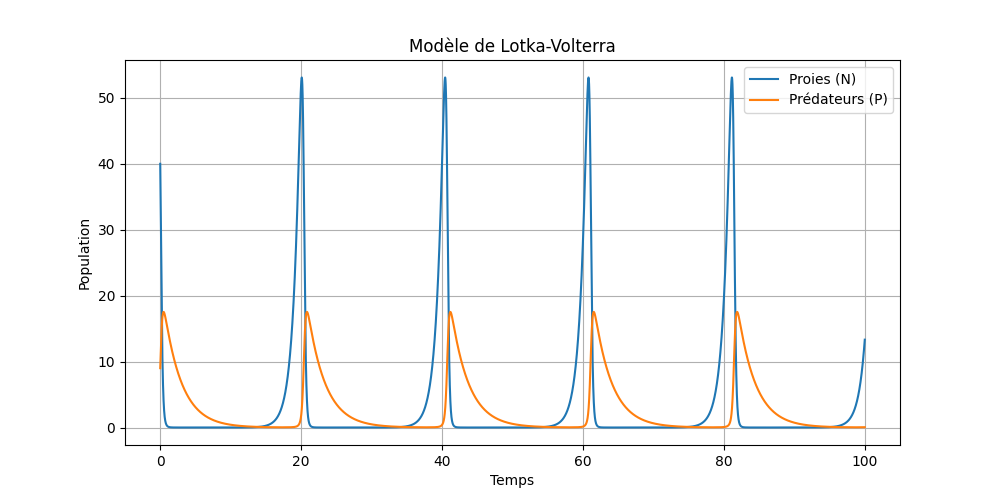
\includegraphics[width=0.4\textwidth]{img/ltka_volterra.png}
    \caption{Evoluions des populations proie et prédateur}
    \label{fig:lotka}
\end{figure}

Nous remarquons que les variations des populations oscillent de manière régulière. En traçant les variations du couple $(N(t), P(t))$ (Figure \ref{fig:phase}), nous observons des solutions périodiques. Les solutions constantes sont les points tels que $N = 0, P = 0$.
\begin{figure}[h]
    \centering
    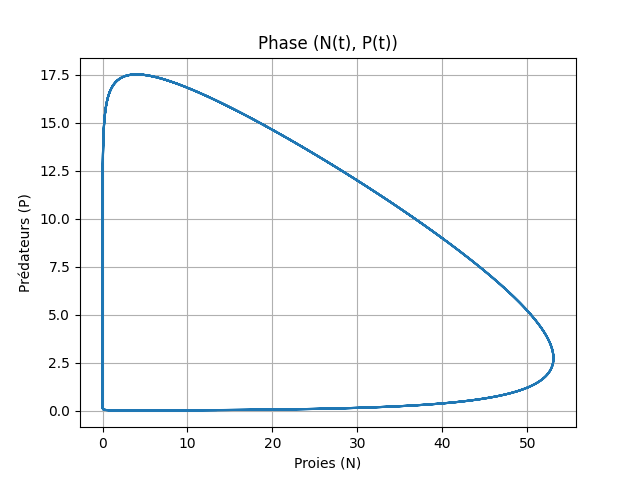
\includegraphics[width=0.4\textwidth]{img/phase.png}
    \caption{Variations du couple $(N(t), P(t))$}
    \label{fig:phase}
\end{figure}
Nous pouvons calculer cette période à l'aide du module \textit{scipy} de Python. Dans l'exemple décrit précédemment, la période est d'environ 20.35.
\subsubsection{Solutions proches du point $y_0$}
Pour un point $y_0$, nous pouvons calculer les variations entre les solutions partant de conditions initiales proches.
Comme présenté sur la figure \ref{fig:local_y0} pour le point initial $(1, 1)$. On remarque que les solutions forment un cercle autour du point.
Nous remarquons également que la forme du diagramme dépend du point initial. 
\begin{figure}[h]
    \centering
    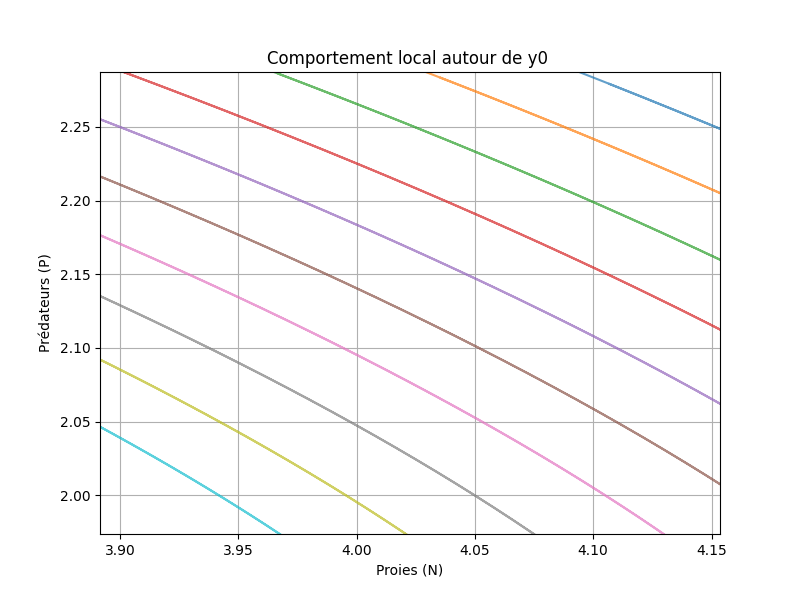
\includegraphics[width=0.4\textwidth]{img/local_y0.png}
    \caption{Variations du couple $(N(t), P(t))$}
    \label{fig:local_y0}
\end{figure}
\subsubsection{Points singuliers}
Nous pouvons calculer des solutions constantes en étudiant les valeurs de $t$ telles que $\frac{dN(t)}{dt} = 0, \frac{dP(t)}{dt} = 0$.\\
On trouve des solutions constantes lorsque $N = 0, P = 0$, également lorsque $N = \frac{d}{c}, P = \frac{a}{b}$.
Nous remarquons que les solutions autour d'un point singulier forment une série autour du point.

